% !TEX root = main.tex
% !TEX root = main.tex
\documentclass[letterpaper, 11pt]{extarticle}
% \usepackage{fontspec}

% ==================================================

% document parameters
% \usepackage[spanish, mexico, es-lcroman]{babel}
\usepackage[english]{babel}
\usepackage[margin = 1in]{geometry}

% ==================================================

% Packages for math
\usepackage{mathrsfs}
\usepackage{amsfonts}
\usepackage{amsmath}
\usepackage{amsthm}
\usepackage{amssymb}
\usepackage{physics}
\usepackage{dsfont}
\usepackage{esint}

% ==================================================

% Packages for writing
\usepackage{enumerate}
\usepackage[shortlabels]{enumitem}
\usepackage{framed}
\usepackage{csquotes}

% ==================================================

% Miscellaneous packages
\usepackage{float}
\usepackage{tabularx}
\usepackage{xcolor}
\usepackage{multicol}
\usepackage{subcaption}
\usepackage{caption}
\captionsetup{format = hang, margin = 10pt, font = small, labelfont = bf}

% Citation
\usepackage[round, authoryear]{natbib}

% Hyperlinks setup
\usepackage{hyperref}
\definecolor{links}{rgb}{0.36,0.54,0.66}
\hypersetup{
   colorlinks = true,
    linkcolor = black,
     urlcolor = blue,
    citecolor = blue,
    filecolor = blue,
    pdfauthor = {Author},
     pdftitle = {Title},
   pdfsubject = {subject},
  pdfkeywords = {one, two},
  pdfproducer = {LaTeX},
   pdfcreator = {pdfLaTeX},
   }

% \begin{document}
% Hello, world! This is a minimal document to test the preamble.
% \end{document}

\usepackage{listings} 
\usepackage{xcolor}

\definecolor{codegreen}{rgb}{0.12,0.6,0.33}
\definecolor{codegray}{rgb}{0.5,0.5,0.5}
\definecolor{codepurple}{rgb}{0.58,0,0.82}
\definecolor{codeblue}{rgb}{0,0.1,0.8}
\definecolor{backcolour}{rgb}{0.95,0.95,0.92}

\lstdefinestyle{pythonstyle}{
   backgroundcolor=\color{backcolour},
   commentstyle=\color{codegreen},
   keywordstyle=\color{codeblue}\bfseries,
   numberstyle=\tiny\color{codegray},
   stringstyle=\color{codepurple},
   basicstyle=\ttfamily\footnotesize,
   breakatwhitespace=false,
   breaklines=true,
   captionpos=b,
   keepspaces=true,
   numbers=left,
   numbersep=5pt,
   showspaces=false,
   showstringspaces=false,
   showtabs=false,
   tabsize=4,
   language=Python
}

% \usepackage{minted}

\usepackage{titlesec}
\usepackage[many]{tcolorbox}

% Adjust spacing after the chapter title
\titlespacing*{\chapter}{0cm}{-2.0cm}{0.50cm}
\titlespacing*{\section}{0cm}{0.50cm}{0.25cm}

% Indent 
\setlength{\parindent}{0pt}
\setlength{\parskip}{1ex}

% --- Theorems, lemma, corollary, postulate, definition ---
% \numberwithin{equation}{section}

\newtcbtheorem[]{problem}{Problem}%
    {enhanced,
    colback = black!5, %white,
    colbacktitle = black!5,
    coltitle = black,
    boxrule = 0pt,
    frame hidden,
    borderline west = {0.5mm}{0.0mm}{black},
    fonttitle = \bfseries\sffamily,
    breakable,
    before skip = 3ex,
    after skip = 3ex
}{problem}

\tcbuselibrary{skins, breakable}

% --- You can define your own color box. Just copy the previous \newtcbtheorm definition and use the colors of yout liking and the title you want to use.
% --- Basic commands ---
%   Euler's constant
\newcommand{\eu}{\mathrm{e}}

%   Imaginary unit
\newcommand{\im}{\mathrm{i}}

%   Sexagesimal degree symbol
\newcommand{\grado}{\,^{\circ}}

% --- Comandos para álgebra lineal ---
% Matrix transpose
\newcommand{\transpose}[1]{{#1}^{\mathsf{T}}}

%%% Comandos para cálculo
%   Definite integral from -\infty to +\infty
\newcommand{\Int}{\int\limits_{-\infty}^{\infty}}

%   Indefinite integral
\newcommand{\rint}[2]{\int{#1}\dd{#2}}

%  Definite integral
\newcommand{\Rint}[4]{\int\limits_{#1}^{#2}{#3}\dd{#4}}

%   Dot product symbol (use the command \bigcdot)
\makeatletter
\newcommand*\bigcdot{\mathpalette\bigcdot@{.5}}
\newcommand*\bigcdot@[2]{\mathbin{\vcenter{\hbox{\scalebox{#2}{$\m@th#1\bullet$}}}}}
\makeatother

%   Hamiltonian
\newcommand{\Ham}{\hat{\mathcal{H}}}

%   Trace
\renewcommand{\Tr}{\mathrm{Tr}}

% Christoffel symbol of the second kind
\newcommand{\christoffelsecond}[4]{\dfrac{1}{2}g^{#3 #4}(\partial_{#1} g_{#2 #4} + \partial_{#2} g_{#1 #4} - \partial_{#4} g_{#1 #2})}

% Riemann curvature tensor
\newcommand{\riemanncurvature}[5]{\partial_{#3} \Gamma_{#4 #2}^{#1} - \partial_{#4} \Gamma_{#3 #2}^{#1} + \Gamma_{#3 #5}^{#1} \Gamma_{#4 #2}^{#5} - \Gamma_{#4 #5}^{#1} \Gamma_{#3 #2}^{#5}}

% Covariant Riemann curvature tensor
\newcommand{\covariantriemanncurvature}[5]{g_{#1 #5} R^{#5}{}_{#2 #3 #4}}

% Ricci tensor
\newcommand{\riccitensor}[5]{g_{#1 #5} R^{#5}{}_{#2 #3 #4}}

\begin{document}

\textsf{\LARGE{\textbf{Take-home exam 1}}}

\normalsize{\textit{Dynamical Systems}}

\vspace{1ex}

\textsf{\textbf{Student:}} \text{Males-Araujo Yorlan}, 
\href{mailto:yorlan.males@yachaytech.edu.ec}{\texttt{yorlan.males@yachaytech.edu.ec}}\\
\textsf{\textbf{Lecturer:}} \text{Mario Cosenza}, 
\href{mcosenza@yachaytech.edu.ec}{\texttt{mcosenza@yachaytech.edu.ec}}

Yachay Tech, \today.

\vspace{2ex}

\begin{problem}{Classification of fixed points}{problem-label}
A particle of mass $m = 1$ is moving in the potential $V(x) = - (1/2)x^2 + (1/4)x^4$.
Find and classify the fixed points (node, saddle, focus) according to their stability.
\end{problem}

We need to use the Hamiltonian formalism for this problem.
As such, we first write
\[
    \label{eq:hamiltonian}
    H(x, p) = T + V = \frac{p^2}{2} - \frac{1}{2}x^2 + \frac{1}{4}x^4,
\]

which is used to find the equations of motion
\[
    \label{eq:hamiltonian_eqs}
    \begin{aligned}
        \dot{x} &= +\frac{\partial H}{\partial p} = p,\\
        \dot{p} &= -\frac{\partial H}{\partial x} = x - x^3 = x(1 - x^2).
    \end{aligned}
\]

The fixed points are obtained by setting them to zero and
solving
\[
    \begin{aligned}
        0 &= p^*,\\
        0 &= x(1 - x^2) \implies x^* = 0, \pm 1.
    \end{aligned}
\]

They combine to give us
\[
    \begin{aligned}
        \textbf{x}_0^* &= (0, 0),\\
        \textbf{x}_1^* &= (1, 0),\\
        \textbf{x}_2^* &= (-1, 0).
    \end{aligned}
\]

In order to do the classification, we need to 
calculate the Jacobian matrix. In our case,
\[
    J = \begin{bmatrix}
        \displaystyle\frac{\partial \dot{x}}{\partial x} & \displaystyle\frac{\partial \dot{x}}{\partial p}\\[2.5ex]
        \displaystyle\frac{\partial \dot{p}}{\partial x} & \displaystyle\frac{\partial \dot{p}}{\partial p}
    \end{bmatrix} =
    \begin{bmatrix}
        0 & 1\\
        1 - 3x^2 & 0
    \end{bmatrix}.
\]

By evaluating the Jacobian at the points found, we obtain the
eigenvalues for each
\[
    \begin{aligned}
        J(\textbf{x}_0^*) &= \begin{bmatrix}
            0 & 1\\
            1 & 0
        \end{bmatrix} \implies \lambda^2 - 1 = 0 \implies \lambda = \pm 1\\
        J(\textbf{x}_1^*) &= \begin{bmatrix}
            0 & 1\\
            -2 & 0
        \end{bmatrix} \implies \lambda^2 +2=0 \implies \lambda = \pm i\sqrt{2}.
    \end{aligned}
\]
Since $J(\textbf{x}_1^*) = J(\textbf{x}_2^*)$, we have them all and
we can proceed with the classification:

\begin{itemize}[label=\textbf{--}]
    \item $\textbf{x}_0^*$ is a saddle because it has real eigenvalues
    with opposite sign.
    \item $\textbf{x}_1^*$ and $\textbf{x}_2^*$ are limit cycles because
    their eigenvalues are purely imaginary.
\end{itemize}

All in all,
\[
\boxed{
    \begin{aligned}
        \textbf{x}_0^* &= (0, 0) \rightarrow \text{ saddle},\\
        \textbf{x}_1^* &= (1, 0) \rightarrow \text{ limit cycle},\\
        \textbf{x}_2^* &= (-1, 0) \rightarrow \text{ limit cycle}.
    \end{aligned}
}
\]


\begin{problem}{Hopf bifurcation}{problem-label-2}
Consider the system $\ddot{x} + \lambda(x^2 - 1)\dot{x} + x - a = 0$.
Find the curves on the space of parameters $(\lambda, a)$ where a Hopf bifurcation occurs.
\end{problem}

We start by rewriting the equation as a system of first-order ODEs. We define
\[
    \textbf{S}(t) = \begin{bmatrix}
        x_1\\
        x_2
    \end{bmatrix} = \begin{bmatrix}
        x\\
        \dot{x}
    \end{bmatrix},
\]
so that
\[
    \frac{d\textbf{S}}{dt} = \begin{bmatrix}
        \dot{x}_1\\
        \dot{x}_2
    \end{bmatrix}=\begin{bmatrix}
        x_2\\
        -\lambda(x_1^2 - 1)x_2 - x_1 + a
    \end{bmatrix}.
\]
We have to look for the fixed points now. The first equation yields $x_2^*=0$, and
we can plug it into the second one:
\[
    0 = - x_1^* + a \implies x_1^* = a.
\]
So the fixed points are $\textbf{x}^*=(a,0)$. We can proceed with the Jacobian matrix,
\[
    J = \begin{bmatrix}
        0 & 1\\
        -2\lambda x_1 x_2 - 1 & -\lambda(x_1^2 - 1)
    \end{bmatrix},
\]
and evaluate it at the fixed point
\[
    J(\textbf{x}^*) = \begin{bmatrix}
        0 & 1\\
        -1 & -\lambda(a^2 - 1)
    \end{bmatrix}.
\]
Then, the characteristic equation is
\[
    \omega^2 + \lambda(a^2 - 1)\omega + 1 = 0,
\]
whose roots are
\[
    \omega_{1,2} = \frac{-\lambda(a^2 - 1) \pm i\sqrt{4-\lambda^2(a^2 - 1)^2}}{2},
\]
assuming $4-\lambda^2(a^2 - 1)^2>0$, so that $\omega_1=\omega_2^*$. Furthermore, a Hopf bifurcation occurs
when the eigenvalues cross the imaginary axis, which happens when the real part of the eigenvalues changes
sign. In this system, this occurs when
\[
    \lambda(a^2 - 1) = 0 \implies a^2 = 1.
\]
We ommit the case when $\lambda = 0$ because it would take $\dot{x}$ away from the ODE. Therefore, the bifurcation
happens at the curves
\[
\boxed{
    \begin{aligned}
        a &= 1,\\
        a &= -1,
    \end{aligned}
}
\]
when limited by $4-\lambda^2(a^2 - 1)^2>0$.

\begin{problem}{Fractal dimension}{problem-label-3}
Calculate the fractal dimension of the following object
shown at three successive levels of construction.

\begin{center}
    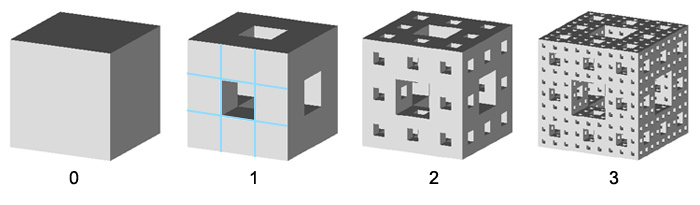
\includegraphics[scale=0.5]{images/cube_fractal.jpg}
\end{center}
\end{problem}

We observe that the object has been broken into 20 pieces, 
and each piece would need to be scaled by a factor of 3
to obtain the original object. Then,

\[
\boxed{
    D = \frac{\log{N}}{\log{\epsilon}} = \frac{\log{20}}{\log{3}} \approx 2.7268,
}
\]
which is less than 3, as expected.


\begin{problem}{Sensitivity and analytical solution}{problem-label-4}

    Consider the map $x_{n+1} = f(x_n) = (2x_n^{2/3} - 1)^3$ , for $x_n \in [-1, 1]$.

    \begin{enumerate}[(a)]
        \item Show, by iterating two close initial conditions, that this map is chaotic.
        \item Show that $x_n = \cos^3 (2^n \cos^{-1} (x_0^{1/3}))$ is a solution $\forall n$.
    \end{enumerate}

\end{problem}

\begin{enumerate}[(a)]
    \item In python, we coded this simple function that implements
    the map and returns the evolution given an initial condition:
    \begin{lstlisting}[style=pythonstyle]
    # Simple function
    def map(x0: float, iter: int) -> list:
        """
        Computes the evolution of an initial condition.

        Parameters
        ----------
        x0 : float
            Initial condition.
        iter : int
            Number of iterations

        Returns
        -------
        x : list
            Evolution of the initial condition.
        """
        # Add the first element
        x = [x0]

        # Iteration process
        for i in range(iter + 1):
            
            # Compute next element
            next = (2 * x[i] - 1)**3

            # Save it
            x.append(next)

        return x
    \end{lstlisting}

    Then we just chose two \textit{extremely} close initial conditions (denoted $x_0$ and $x_1$),
    and found the map evolutions:
    \begin{lstlisting}[style=pythonstyle]
    # Initial conditions
    x0 = 0.9999999998
    x1 = 0.9999999999

    # Iterate!
    x0_evol = map(x0, iter = 14)
    x1_evol = map(x1, iter = 14)
    \end{lstlisting}

    % Figure
    \begin{figure}[!ht]
        \centering
        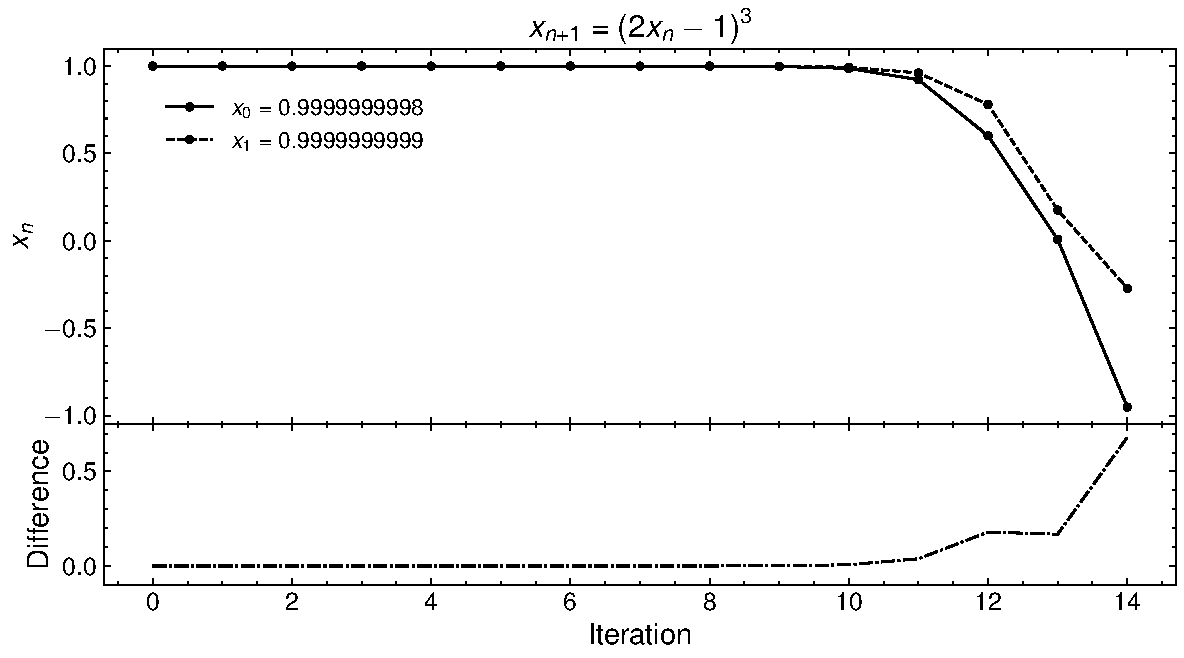
\includegraphics[scale=0.6]{images/4a.pdf}
        \captionof{figure}{Evolution of two close initial conditions, plus
        the difference between them.}
        \label{fig:4a}
    \end{figure}

    The results can be seen in figure \ref{fig:4a}. They evolve together
    for the first 10 iterations, but, in the 11th iteration, they start to separate. 
    It takes little time for them to do so, even though they were very close
    at the beginning. \boxed{\text{This is a clear sign of chaos.}}


    \item We'll do it by induction, starting by plugging the expression in the map
    \[
        x_{n+1} = [2(\cos^3 (2^n \cos^{-1} (x_0^{1/3}))^{2/3} - 1]^3.
    \]
    Then, some straightforward algebra gives us
    \[
    \begin{aligned}
        x_{n+1} &= [2\cos^2 (2^n \cos^{-1} (x_0^{1/3})) - 1]^3\\
        &= [2\cos^2 (2\cdot 2^{n-1} \cos^{-1} (x_0^{1/3})) - 1]^3.
    \end{aligned}
    \]
    We can now apply the identity $\cos^2(2x)=(1+\cos(4x))/2$,
    resulting in
    \[
    \begin{aligned}
        x_{n+1} &= \left[2\cdot\frac{1 + \cos(2^2\cdot 2^{n-1} \cos^{-1} (x_0^{1/3}))}{2}-1\right]^3\\
        &= \left[\cos(2^{n+1} \cos^{-1} (x_0^{1/3}))\right]^3\\
        &= \cos^3 (2^{n+1} \cos^{-1} (x_0^{1/3})).
    \end{aligned}
    \]
    Thus, the expression holds for $n+1$. To finish, let's verify the base case
    \[
        x_0 = \cos^3 (2^0 \cos^{-1} (x_0^{1/3})) = \cos^3 (\cos^{-1} (x_0^{1/3})) = x_0^{3/3} = x_0.
    \]

    \boxed{
        \text{Therefore, } x_n = \cos^3 (2^n \cos^{-1} (x_0^{1/3})) \text{ is a solution } \forall n.
    }

\end{enumerate}

\begin{problem}{Bifurcation diagram and Lyapunov exponent}{problem-label-5}
    Consider the map $x_{n+1} = f(x_n) = \sin^2(r\,\arcsin{\sqrt{x_n}})$, for $x_n \in [0, 1]$.

    \begin{enumerate}[(a)]
        \item Obtain the bifurcation diagram of $x_n$ as a function of $r$,
        for $r \in [1, 4]$.
        \item Calculate the Lyapunov exponent as a function of $r$, for $r \in [1, 4]$.
    \end{enumerate}

\end{problem}

\begin{enumerate}[(a)]

    \item Once passed the transient regime, we recorded the data points
    for $r$ in the specified range. For plotting, thanks to the helpful description
    by \cite{WikiTentMap}, we were able to get a good-looking diagram using a
    matrix to store the values of $x_n$ and $r$, which allowed us to control
    the resolution in a simple yet effective manner. The result is shown in figure
    \ref{fig:5a}.

    \begin{figure}[!ht]
        \centering
        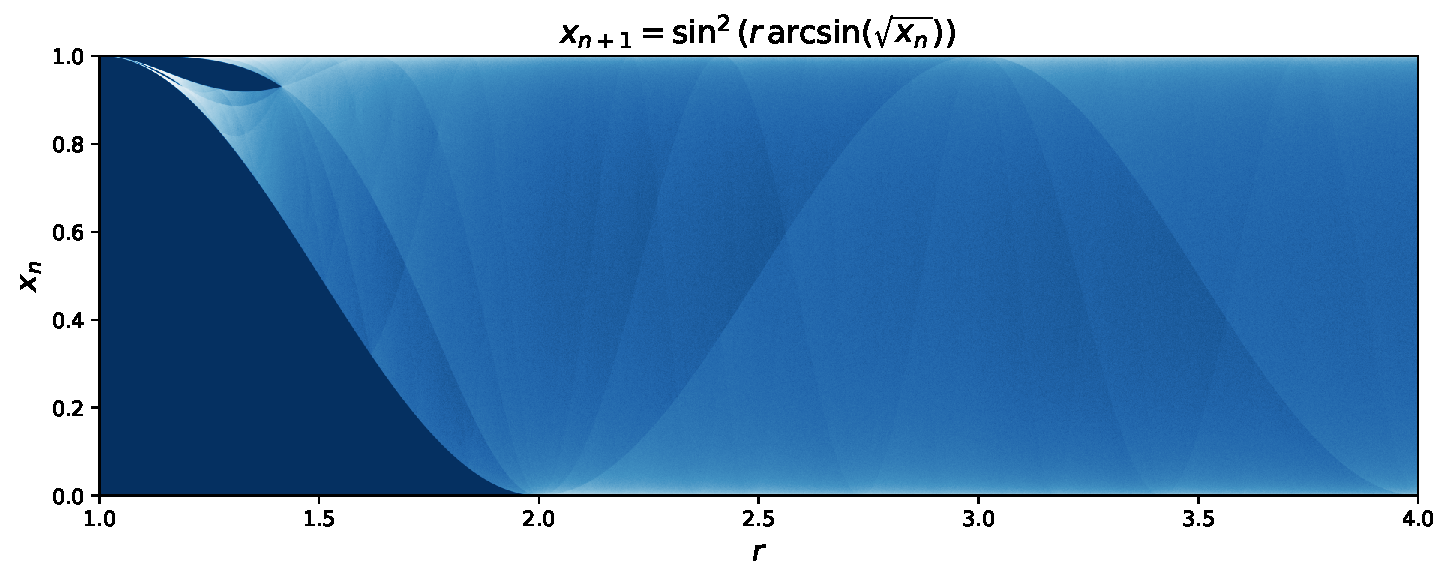
\includegraphics[scale=0.65]{images/5a[1-4].pdf}
        \captionof{figure}{Bifurcation diagram for $r \in [1, 4]$.}
        \label{fig:5a}
    \end{figure}
    

    It clearly shows transition to chaos by \textit{period doubling}, and, interesting
    aspect, sinusoidal-like curves, indicating points that are not being visited.
    \item To calculate the Lyapunov exponent, we used the formula
    \[
        \lambda = \lim_{n \to \infty} \frac{1}{n} \sum_{i=0}^{n-1} \log{|f'(x_i)|},
    \]
    and, in our case, we have
    \[
        f'(x) = \frac{r\sin{\left(2r\arcsin{\sqrt{x}}\right)}}{2\sqrt{x(1-x)}}.
    \]
    In the implementation, we added small offsets both in the logarithm and 
    derivative denominator to avoid division-by-zero errors. The results are shown
    in figure \ref{fig:5b}.

    \begin{figure}[!ht]
        \centering
        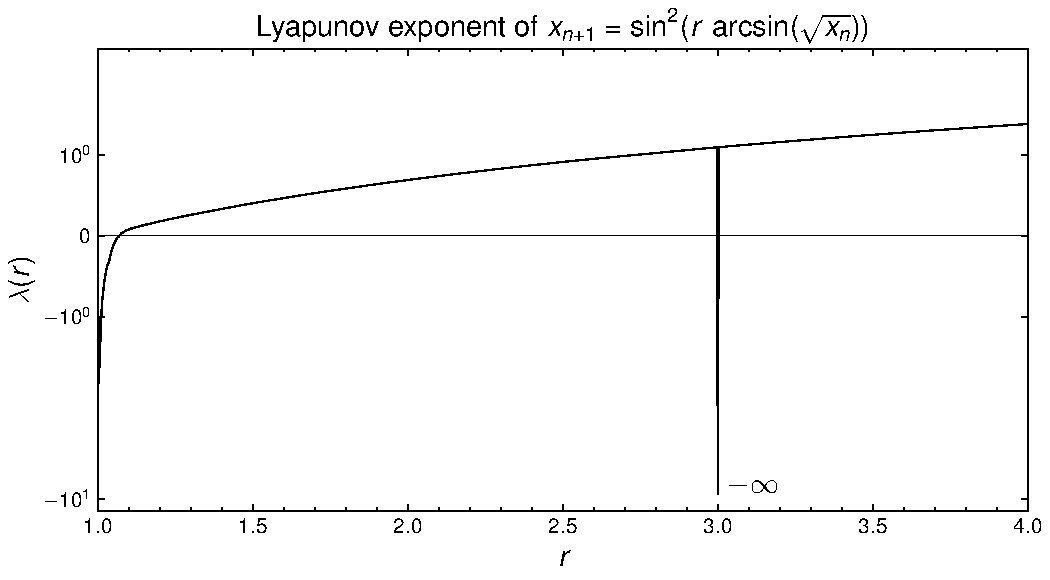
\includegraphics[scale=0.75]{images/5b[1-4].pdf}
        \captionof{figure}{Lyapunov exponent for $r \in [1, 4]$.}
        \label{fig:5b}
    \end{figure}

    We could have forseen the results just by looking at the bifurcation diagram. That is, negative
    for a very small range of $r$ at the beginning, and then increasingly positive for the rest
    of it.

    \textbf{Note}: When solving the problem, we came across an interesting finding: the map
    is \textit{not} chaotic for $r = 3.0$ and $x_0 = 0.250$. This is shown in figure \ref{fig:5c}, where
    we plotted the nontransient evolution of such conditions.     The Lyapunov exponent for this case goes to negative infinity!


    \begin{figure}[!ht]
        \centering
        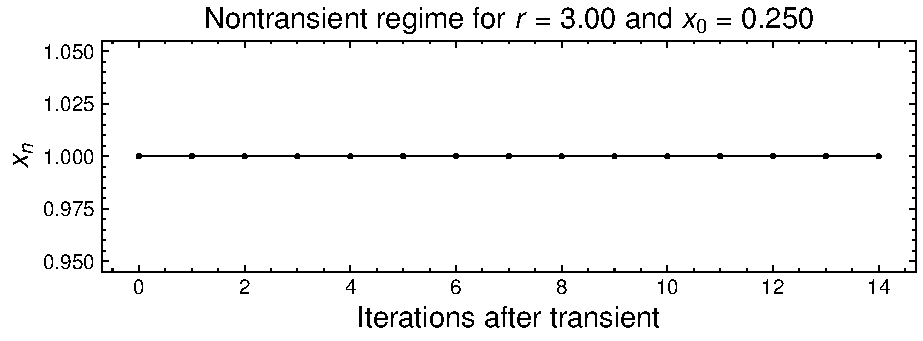
\includegraphics[scale=0.65]{images/not-chaotic.pdf}
        \captionof{figure}{Strange non-chaotic behaviour for specific conditions.}
        \label{fig:5c}
    \end{figure}


\end{enumerate}
\newpage
\begin{problem}{Phase space}{problem-label-6}

    The evolution of a system is described by the following equation:
    \[
        \dddot{x} + a\ddot{x}+\dot{x}-|x|+1=0, \text{ for } a > 0.
    \]

    \begin{enumerate}[(a)]
        \item Find the fixed points of this system.
        \item Plot the attractor of this system in its phase space for $a = 0.6$.
        Is it strange?
        \item Show that this system is not chaotic for $a = 0.68$.
    \end{enumerate}

\end{problem}

\begin{enumerate}[(a)]
    \item We first need to convert the third-order ODE into a system of three first-order ODEs. 
    We do this by defining the state vector
    \[
        \textbf{S}(t) = \begin{bmatrix}
            x_1\\
            x_2\\
            x_3
        \end{bmatrix} = \begin{bmatrix}
            x\\
            \dot{x}\\
            \ddot{x}
        \end{bmatrix},
    \]
    and writing the system of ODEs as
    \[
        \frac{d\textbf{S}}{dt} = \begin{bmatrix}
            x_2\\
            x_3\\
            -a x_3 - x_2 + |x_1| - 1
        \end{bmatrix}.
    \]
    Similarly as before, we set each equation to zero and solve for the fixed points:
    \[
        \begin{aligned}
            0 &= x_2,\\
            0 &= x_3,\\
            0 &= -a x_3 - x_2 + |x_1| - 1.
        \end{aligned}
    \]
    Now, plugging the first two in the third one gives us
    \[
        0 = |x_1| - 1 \implies x_1 = \pm 1.
    \]
    Thus, the fixed points are
    \[\boxed{
        \begin{aligned}
            \textbf{x}_0^* &= (1, 0, 0),\\
            \textbf{x}_1^* &= (-1, 0, 0).
        \end{aligned}
    }
    \]

    \item Rewriting the ODE as a system of first-order ODEs
    is also useful for solving it \textit{numerically}. In python, we started by creating 
    a function that implements such system:

    \begin{lstlisting}[style=pythonstyle]
    # Little function
    def system(t: float, S: np.ndarray, a: float) -> np.ndarray:
        """
        System of first-order ODEs.

        Parameters
        ----------
        t : float
            Time.
        S : np.ndarray
            State vector.
        a : float
            Parameter.

        Returns
        -------
        np.ndarray
            Derivative of the state vector.
        """
        # Extract variables
        x1, x2, x3 = S

        # Define the equations
        dx1_dt = x2
        dx2_dt = x3
        dx3_dt = -a * x3 - x2 + abs(x1) - 1

        return [dx1_dt, dx2_dt, dx3_dt]
    \end{lstlisting}

    After doing that, we called the \texttt{solve\_ivp} function from the \texttt{scipy}
    library to solve the system of equations:

    \begin{lstlisting}[style=pythonstyle]
        # Set a
        a = 0.60

        # Time span and evaluation
        t_span = (0, 1000)
        t_eval = np.linspace(t_span[0], t_span[1], 15000)

        # Initial conditions
        S0 = [0.1, 0.1, 0.1]

        # And solve the system!
        sol = solve_ivp(slope, t_span, S0, t_eval, method='RK45', args=(a,))

        # Extract the solutions
        x1 = sol.y[0]
        x2 = sol.y[1]
        x3 = sol.y[2]
    \end{lstlisting}

    Finally, we plotted the results in phase space, shown in figure \ref{fig:6b}. For
    visualization purposes, we didn't include the first part of the evolution, and also added 
    a small set of axes indicating the orientation. I think it came out pretty well.
    \begin{figure}[!ht]
        \centering
        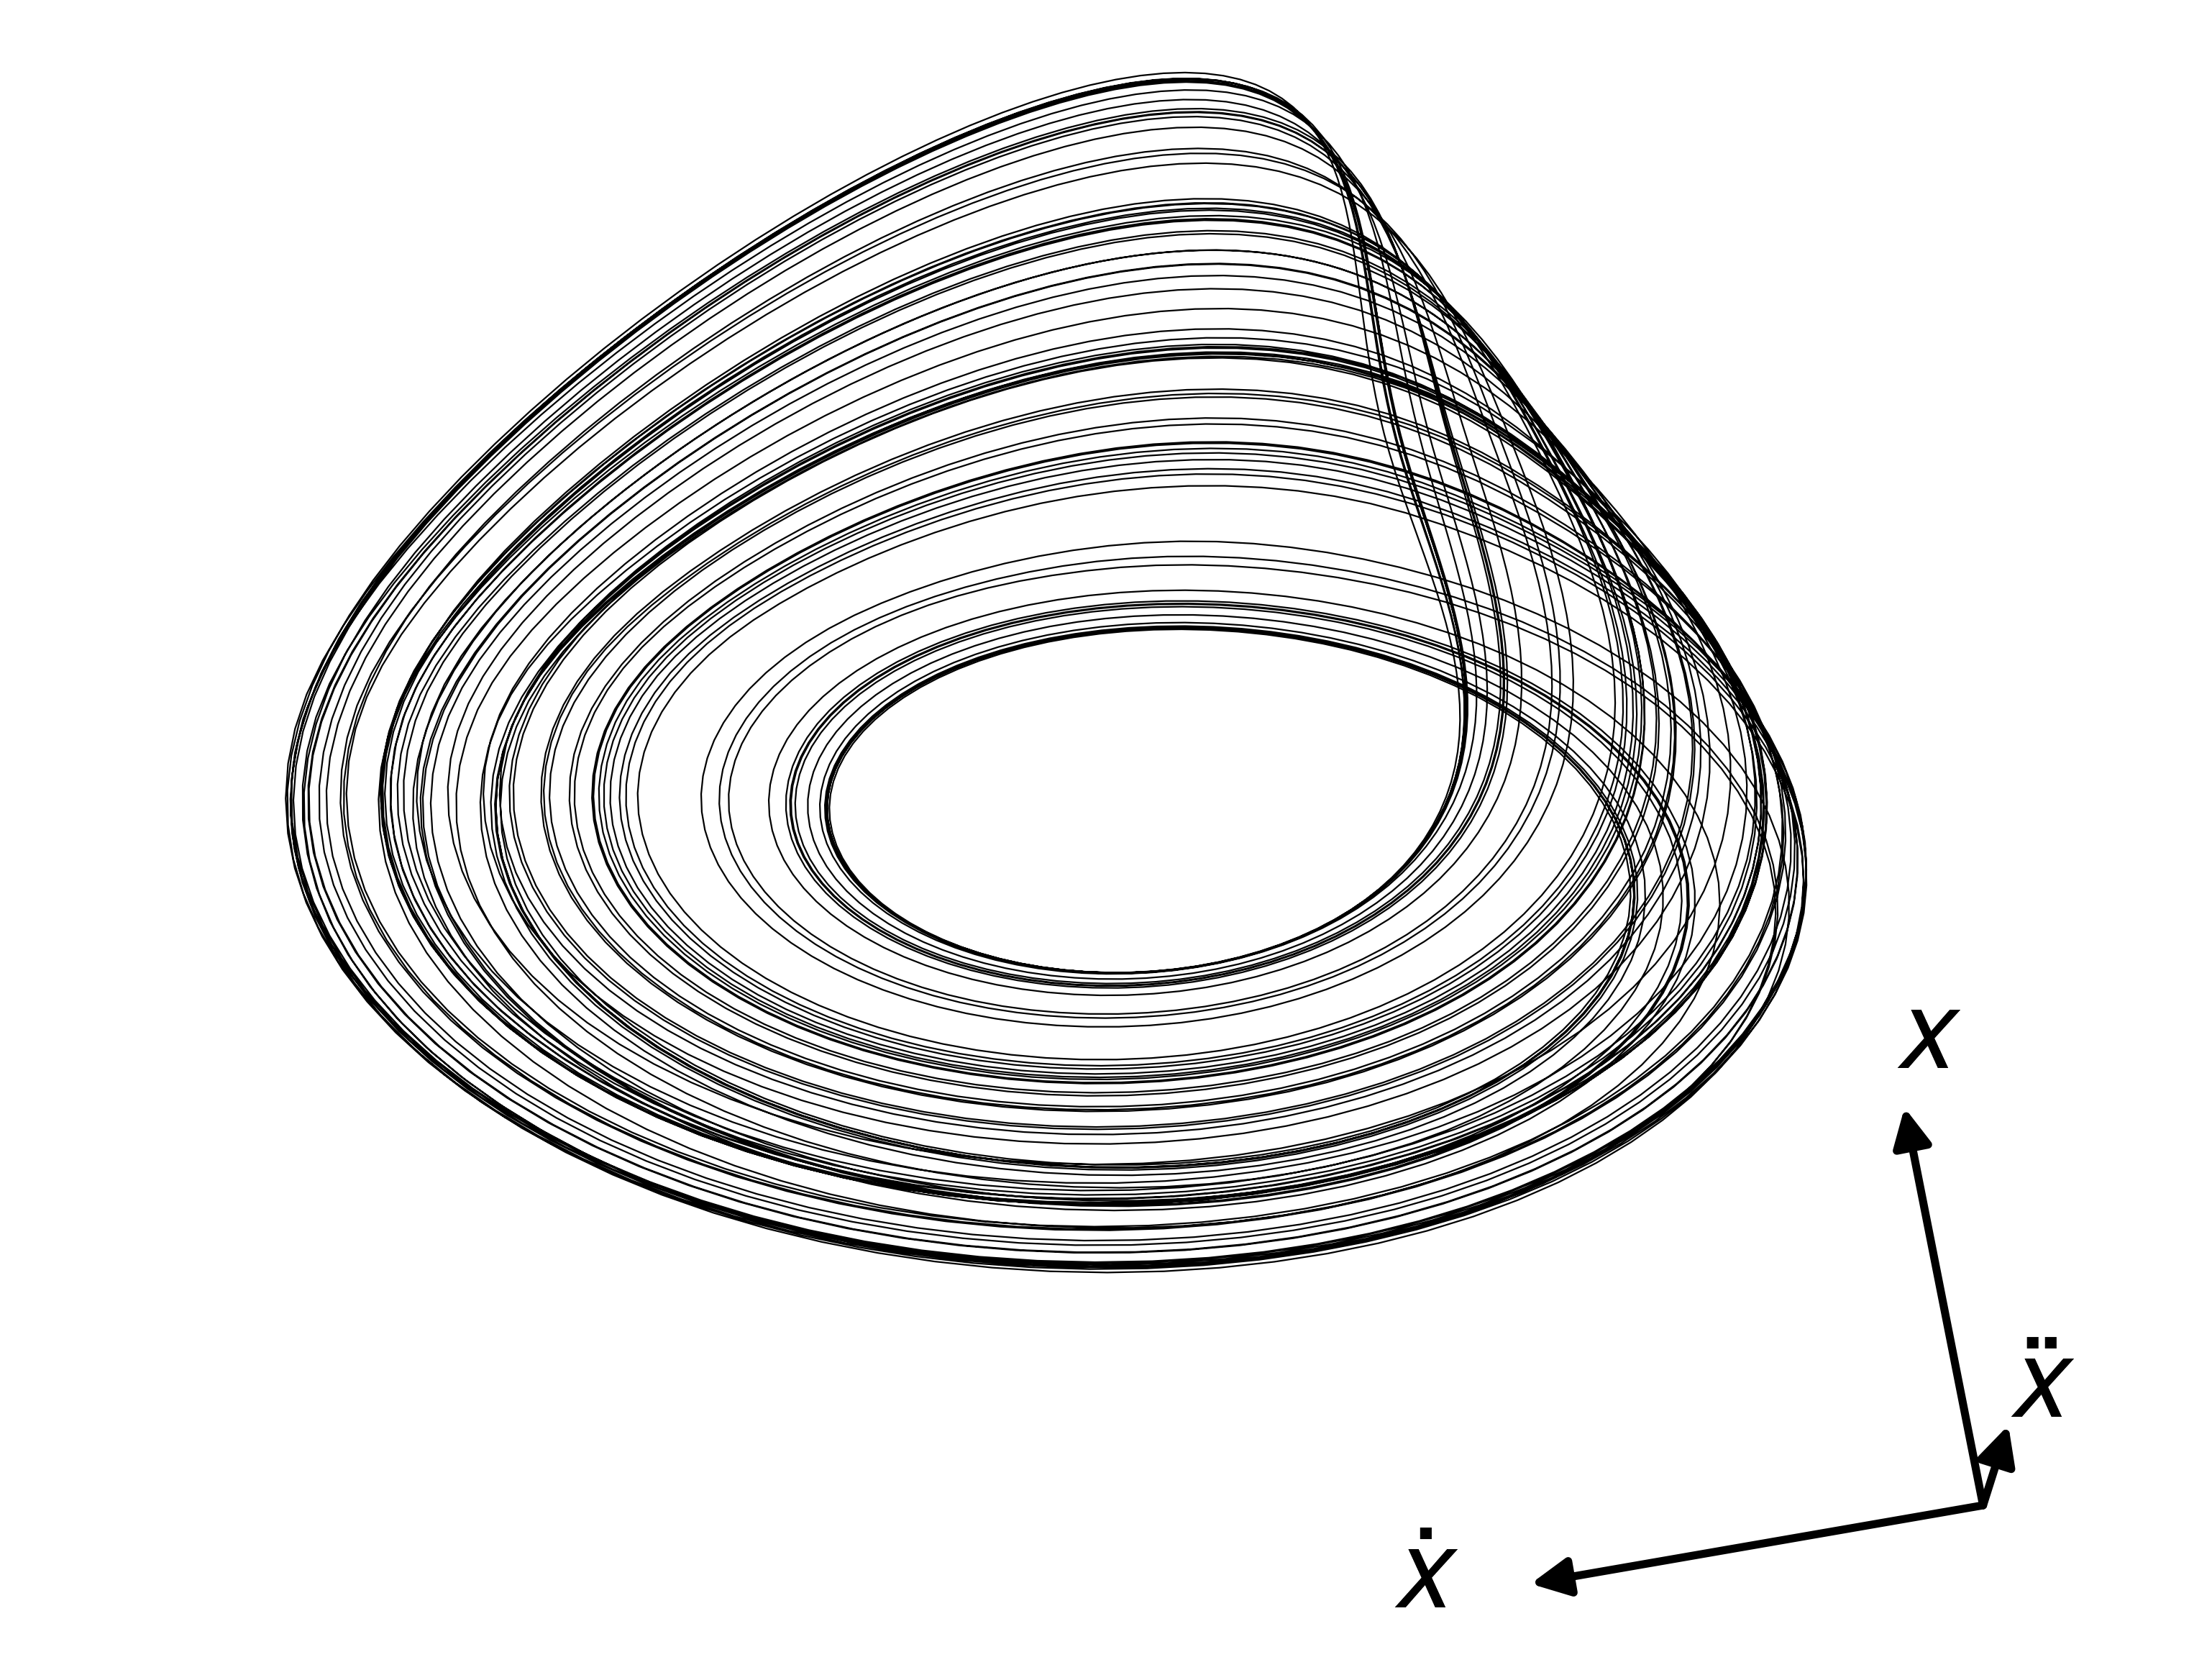
\includegraphics[scale=0.10]{images/6b.png}
        \captionof{figure}{Good view of the system evolution in phase space for $a = 0.60$.}
        \label{fig:6b}
    \end{figure}

    To some degree, it resembles Rossler's attractor. \boxed{\text{Answering, it is indeed of \textit{strange} type.}}

    \item Reusing the same code, we set $a = 0.68$ and the plot
    is shown in figure \ref{fig:6c}. 
    \begin{figure}[!ht]
        \centering
        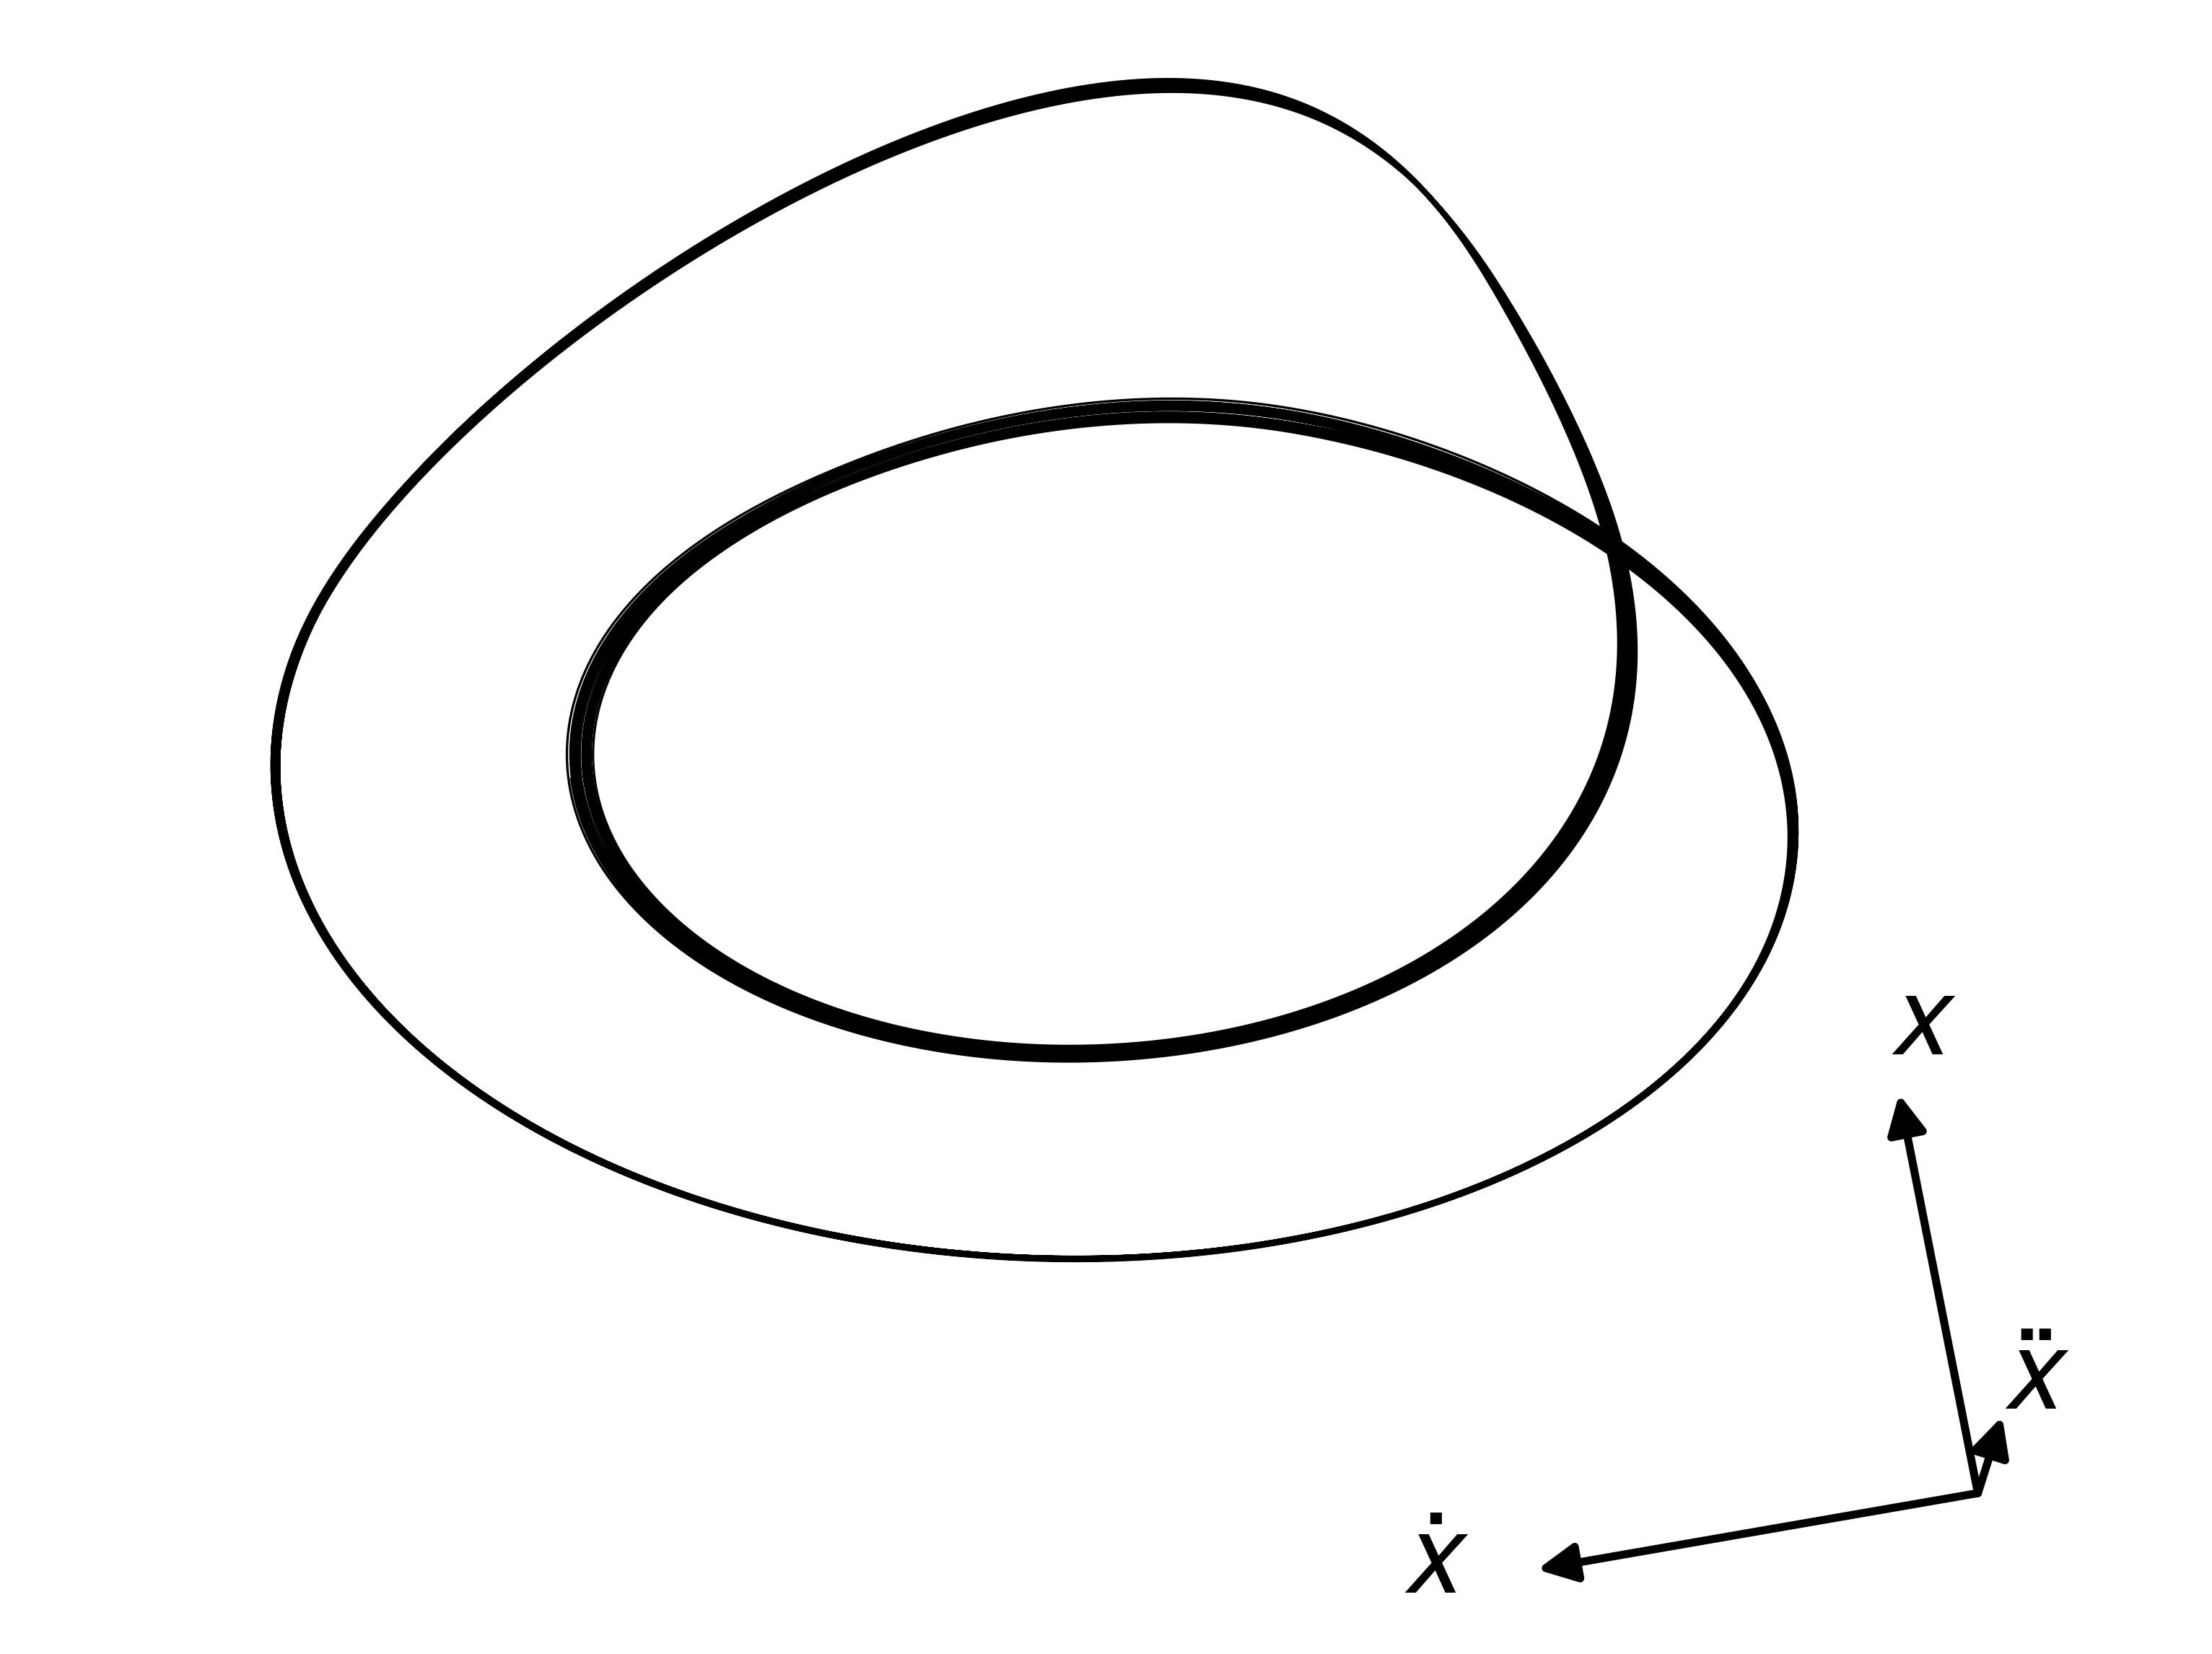
\includegraphics[scale=0.10]{images/6c.png}
        \captionof{figure}{Non-chaotic system evolution in phase space for $a = 0.68$.}
        \label{fig:6c}
    \end{figure}

    The result is quite different from the previous: it looks like
    a \textit{closed curve} in phase space. An evolution like this 
    indicates the system exhibits stable oscillatory behaviour. In
    other words, \boxed{\text{it is not chaotic when $a = 0.68$.}}
\end{enumerate} 

\newpage
\vspace{0.1ex}

\bibliographystyle{apalike}
\bibliography{references}

\end{document}